% Chapter Template

\chapter{Platform Implementation} % Main chapter title

\label{Chapter5} % Change X to a consecutive number; for referencing this chapter elsewhere, use \ref{ChapterX}

\lhead{Chapter 5. \emph{System Implementation}} % Change X to a consecutive number; this is for the header on each page - perhaps a shortened title

\section{Software architecture}
The important components of the system shown in Fig~\ref{fig:architecture} are
\begin{itemize}
\item \textbf{Application Components}
\begin{itemize}
\item \emph{Context}: The application context contains the complete description of the world. It contains latest information about all the robots including their location, sensor data and status. It also contains information about all the humans in the environment along with their active motions/gestures as supplied by the motion recognition modules.
\item \emph{Parameter Server}: The parameter server acts as a central repository for managing the parameters of the system and of the distributed components.
\item Embedded Web Server: The web server embedded in the application serves the file and data requests from the web client.
\item \emph{Context Orchestrator}: The orchestrator collect uptodate information about the robots and humans in the environment from the perception system and updates the Context.
\item \emph{Bootstrapper} : The bootstrapper takes care of initializing the system and starting up all the pre-configured nodes. It also takes of starting and stopping the behavior programs when requested by the user. 
\item \emph{Behavior Program} : A dynamic component that will be created when the user starts the program he/she designed using the user interface. The declarative description of the behavior is parsed in order to create a memory model. The Behavior program node monitors the application context for the motion triggers and invokes the corresponding robot actions according to the way it is being described in the program.
\end{itemize}
\item \textbf{Distributed Components} : These are nodes in the system each with a specific goal that can be started/stopped at any time during the entire application life-cycle without affecting the other nodes or the system. All the nodes will communicate with the application using message passing techniques. They can run in any machine inside the network.
\begin{itemize}
\item \emph{Motion Recognition Node} : A dedicated node that interacts with a motion recognition sensor and sends the detected gestures and motions to the application. Additionally each motion recognition module registers a set of actions/gestures that could be detected with the sensor associated with it.
\item \emph{Robot Interface Node} : A dedicated node that interacts with a specific robot and can invoke a set of actions on it. It also sends periodic update about the Robot status to the application. Moreover it registers a set of actions that could be invoked on the robot associated with it.
\item \emph{Localization Node} : A dedicated node which uses the perception system to resolve and publish the current position of the robot and the human which is very important for interaction.
\end{itemize}
\item \textbf{User Interface}: The user interface is a web application that runs on any latest web-kit browsers supporting WebGL technology. 
\begin{itemize}
\item \emph{Behavior Designer}: The Behavior designer surface could be used by the user to drag and drop the behavior blocks and construct the program using the set of motion capabilities registered by the active motion recognition nodes and the set of robot action capabilities registered by the active robot interface nodes. The behavior designed using the designer will be encoded into a declarative XML format and sent to the server when the user request to start the program. The designer offers a full range of capabilities like Create/Edit/Delete/Save behavior programs.
\item \emph{Visualization}: The visualization could be used to see the interaction of the human and robot inside a virtual 3D environment.
\end{itemize}
\end{itemize}
\begin{figure}
\centering
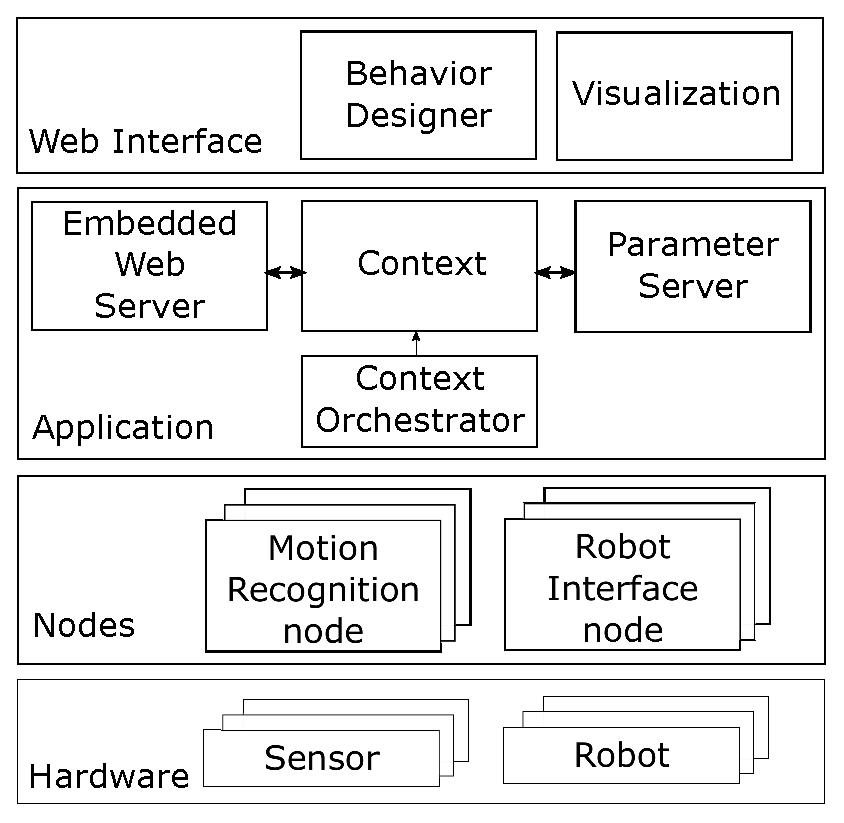
\includegraphics[width=\textwidth]{assets/architecture.eps}
\caption[System Architecture]{System Architecture}
\label{fig:architecture}
\end{figure}